\documentclass[a4paper,12pt]{report}

\usepackage{alltt, fancyvrb, url}
\usepackage{graphicx}
\usepackage[utf8]{inputenc}
\usepackage{float}
\usepackage{hyperref}

\usepackage[italian]{babel}

\usepackage[italian]{cleveref}

\title{\textbf{Elaborato per il corso di Basi Di Dati \\ A.A 2022/2023}}

\author{Ettore Farinelli \\ ettore.fainelli@studio.unibo.it \\ 0001019995}

\date{\today}

\begin{document}

\maketitle

\tableofcontents

\chapter{Analisi dei requisiti}
Si pone l'obbiettivo di realizzare un database capace di gestire un organizzazione di arti marziali come può essere, 
per esempio, \textsc{L'Ultimate Fighting Championship, (UFC)}. La base di dati dovrà quindi essere capace di registrare 
nuovi \textbf{lottatori} e in caso rimuoverli(squalifica, infortuneo, ritiro). Inoltre sarà possibile registrare \textbf{eventi}, 
dove i combattenti si scontreranno aggiornando (dopo gli \textbf{scontri}), gli \textbf{score} dei partecipanti 
e in caso le \textbf{classifiche}.

\section{Intervista}
A seguito di una prima intervista si sono ottenute le seguenti richieste:\medskip

Per ogni partecipante alla lega bisogna tenere traccia del nome, cognome, codice fiscale, data di nascita, team, peso e \textbf{arte 
marziale} in cui vuole lottare. Alla iscrizione di un nuovo lottatore esso verrà inserito all'ultimo 
posto nella classifica della propria categoria. Ci sarà la possibilità di registrare i \textbf{team} dei combattenti tenendo traccia di: nome, amministratore e 
origine. Saranno presenti diverse classifiche per ogni tipo di categoria dove i lottatori saranno ordinati 
in base ai loro \textbf{record} (V, P, S), dove le vittorie assegnano 3 punti, i pareggi 1 e le sconfitte 0.\par
Le categorie in cui verranno suddivisi i membri della lega sono: \textit{Peso Piuma} (fino a 65kg), \textit{Welterweight} 
(65kg - 77kg), \textit{Peso Medio} (77kg - 84kg) e \textit{Pesi Massimi} (da 84kg in poi). Inoltre non ci sarà una vera e propria 
divisione in arti marziali in quanto combattenti praticanti discipline diverse potranno scontrarsi tra loro, le arti marziali sono le 
seguanti: \textit{MMA} (Mixed Martial Arts), \textit{BJJ} (Brazial Jiu Jitsu) e infine \textit{Muay Thai}. Per ogni 
partecipante dovrà essere inserita la disciplina di competenza possibilmente modificabile in futuro (sarà gestito in maniera 
analoga il peso). Inoltre, partecipanti appartenenti a una determinata categoria potranno scontrarsi solo con altri membri 
della stessa. Gli eventi saranno constituiti da almeno 2 combattimenti ciascuno, bisognerà tener traccia del: nome dello stadio, 
luogo (nazione), costo noleggio stadio, spesa staff, data, orario inizio, orario fine, biglietti standard venduti, biglietti 
premium venduti, costo biglietti standard, costo biglietti premium, introiti netti, inoltre sarà necessario poter associare a un 
evento degli sponsor selezionabili tra quelli disponibili che hanno effettuato un contratto con la lega. Ogni lottatore partecipante 
riceverà un pagamento extra e verrà calcolata una quantità di guadagni tramite pubblicità, tutto in base al numero di biglietti 
venduti per l'evento, così da poter calcolare gli introiti dell'evento, il quale verrà aggiunto in una \textsc{History} dove saranno 
immagazzinati tutti gli eventi passati.

\section{Definizioni}
\begin{itemize}
    \item \textbf{Lottatore}: partecipante alla lega.
    \item \textbf{Organizzatore}: amministratore che ha l'accesso al database e le autorizzazioni per gestirlo. 
    \item \textbf{Evento}: un insieme di scontri avente un luogo e una data.
    \item \textbf{Scontro}: un incontro tra due lottatori della stessa categoria.
    \item \textbf{Classifica}: lista numerata in ordine dal partecipante migliore al peggiore in base ai record personali.
    \item \textbf{Arte marziale}: disciplina frequentante da un partecipante.
    \item \textbf{Team}: associazione a cui possono far parte 1 o piu combattenti, ha lo scopo di seguirli durante gli scontri e allenarli.
    \item \textbf{Record}: terna di vittorie, pareggi, sconfitte (V, P, S), ogni prtecipante ha la sua che definisce la sua posizione in 
        classifica.
\end{itemize}

\subsection{Operazioni Amministratore}
\begin{itemize}
    \item Registrare un nuovo lottatore.
    \item Rimuovere un lottatore.
    \item Registrare un nuovo team.
    \item Rimuovere un team.
    \item Aggiungere/Rimuovere uno sponsor.
    \item Registrare uno evento.
    \item Visualizzare le classifiche.
    \item Modificare i dati dei partecipanti.
\end{itemize}

\chapter{Progettazione Concettuale}
\section{Amministratore}
L'amministratore è colui che utilizza effettivamente a livello di applicazione il database, quindi sarà lui che organizzerà tutte  
le altri parti principali del database come i lottatori, gli eventi, i team e le sponsorizzazioni.

\section{Lottatore}
I lottatori sono il cuore dell'intero database, per questo parte tutto dall'entità "lottatore" a cui sarà associata un'entità 
"record" creata in modo tale da poter tener traccia dello score di ogni combattente, inoltre i lottatore potranno o meno far parte 
di un team precedentemente registrato. Infine, ogni lottatore potrà partecipare a uno scontro per ogni evento, 
in questo caso non sono riuscito a gestire (a livello di schema concettuale) il vincolo per il quale due lottatori 
di categorie diverse non possono combattere.

\section{Evento}
Gli eventi sono il principale elemento della lega dal quale proviene il profitto di quest'ultima. Quindi, è importante 
tenerne traccia con un entità "Storico\textunderscore eventi", inoltre ogni evento potrà essere sponsorizzato da uno o più sponsor registrati nella lega.

\section{Scontro}
Gli scontri constituiscono gli eventi e sono formati da due lottatori della stessa categoria, è importante anche che i due partecipanti 
a uno scontro ricevano un pagamento in base alle volontà dell'amministratore.

\section{Schema concettuale finale}
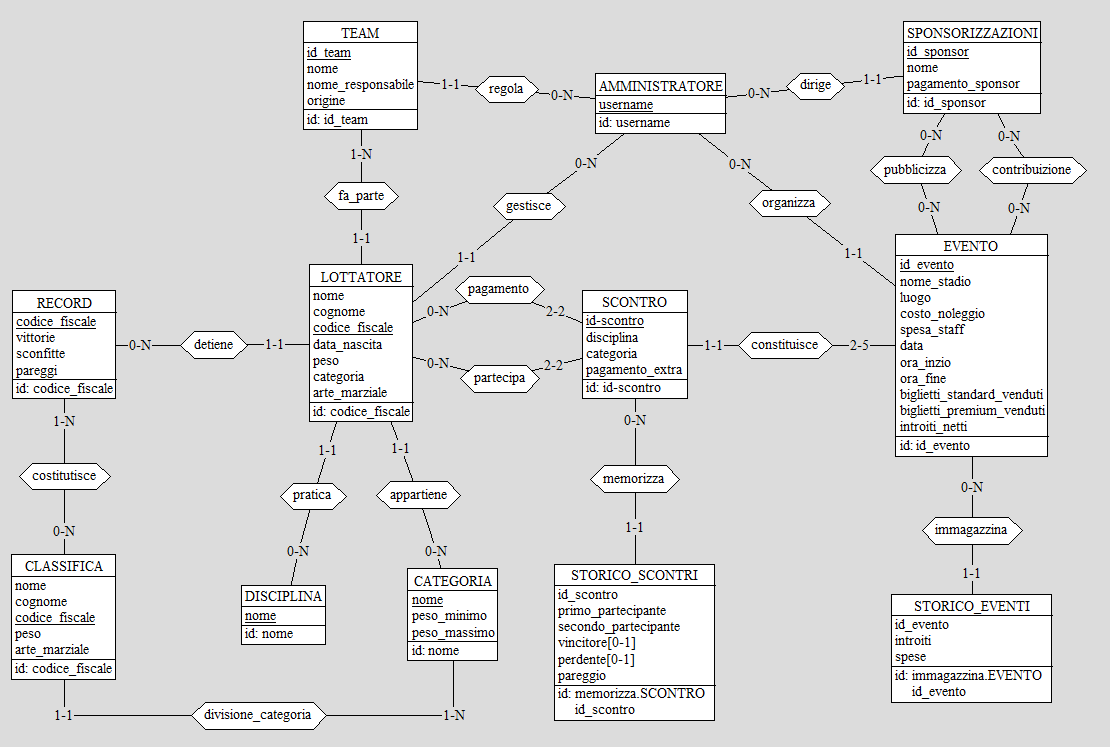
\includegraphics[scale=0.8, angle=90]{./img/schema_finale.png}

\chapter{Progettazione logica}
\section{Stima del volume dei dati}
\begin{itemize}
    \item AMMINISTRATORE: E, 1
    \item LOTTATORE: E, 250
    \item CATEGORIA: E, 4
    \item DISCIPLINA: E, 3
    \item RECORD: E, 250
    \item CLASSIFICA: E, 250
    \item SCONTRO: E, 2000
    \item STORICO\textunderscore SCONTRI: E, 2000
    \item EVENTO: E, 700
    \item STORICO\textunderscore EVENTI: E, 700
    \item SPONSORIZZAZIONI: E, 15
    \item TEAM: E, 150
    \item DIRIGE: A, 20
    \item GESTISCE: A, 350
    \item REGOLA: A, 200
    \item ORGANIZZA: A, 700
    \item DETIENE: A, 250
    \item CONSTITUISCE: A, 250
    \item MEMORIZZA: A, 2000
    \item DIVISIONE\textunderscore CATEGORIA: A, 4
    \item APPARTIENE: A, 250
    \item PRATICA: A, 375
    \item FA\textunderscore PARTE: A, 200
    \item PARTECIPA: A, 4000
    \item PAGAMENTO: A, 4000
    \item CONSTITUISCE: A, 2000
    \item PUBBLICIZZA: A, 3000
    \item CONTRIBUIZIONE: A, 3000
    \item IMMAGAZINA: A, 700
\end{itemize}

\section{Descrizione delle operazioni principali e stima della loro frequenza}
\begin{itemize}
    \item Registrazione nuovo lottatore: 1/10 g
    \item Rimuovere un lottatore: 1/15 g
    \item Registrazione nuovo team: 1/12 g
    \item Rimuovere un team: 1/18 g
    \item Registrare un nuovo sponsor: 1/120 g
    \item Rimuovere uno sponsor: 1/210 g
    \item Registrare un evento: 1/20 g
    \item Visualizzare la classifica: 3/ g
    \item Modificare dati di un partecipante: 1/5 g
\end{itemize} 

\section{Schemi di navigazione e tabelle degli accessi}
\subsection{Registrazione nuovo lottatore}
\begin{table}[H]
    \paragraph{Tavola degli accessi\newline}
    \begin{tabular}{|c|c|c|c|}
    \hline
    Concetto          & Costrutto & Accessi & Tipo \\ \hline
    AMMINISTRATORE    & E         & 1       & R    \\ \hline
    LOTTATORE         & E         & 1       & W    \\ \hline
    RECORD            & E         & 1       & W    \\ \hline
    CLASSIFICA        & E         & 1       & W    \\ \hline
    DETIENE           & A         & 1       & W    \\ \hline
    CONSTITUISCE      & A         & 1       & W    \\ \hline
    GESTISCE          & A         & 1       & R    \\ \hline
    \textit{TOTALE}   &           & 12       &      \\ \hline
    \end{tabular}
\end{table}

\subsection{Rimuovere un lottatore}
\begin{table}[H]
    \paragraph{Tavola degli accessi\newline}
    \begin{tabular}{|c|c|c|c|}
    \hline
    Concetto          & Costrutto & Accessi & Tipo \\ \hline
    AMMINISTRATORE    & E         & 1       & R    \\ \hline
    LOTTATORE         & E         & 1       & W    \\ \hline
    RECORD            & E         & 1       & W    \\ \hline
    CLASSIFICA        & E         & 1       & W    \\ \hline
    DETIENE           & A         & 1       & W    \\ \hline
    CONSTITUISCE      & A         & 1       & W    \\ \hline
    GESTISCE          & A         & 1       & R    \\ \hline
    \textit{TOTALE}   &           & 12      &      \\ \hline
    \end{tabular}
\end{table}

\subsection{Registrazione/Rimozione nuovo team}
\begin{table}[H]
    \paragraph{Tavola degli accessi\newline}
    \begin{tabular}{|c|c|c|c|}
    \hline
    Concetto          & Costrutto & Accessi & Tipo \\ \hline
    AMMINISTRATORE    & E         & 1       & R    \\ \hline
    TEAM              & E         & 1       & W    \\ \hline
    REGOLA            & A         & 1       & R    \\ \hline
    \textit{TOTALE}   &           & 4       &      \\ \hline
    \end{tabular}
\end{table}

\subsection{Registrare/Rimuovere un nuovo sponsor}
\begin{table}[H]
    \paragraph{Tavola degli accessi\newline}
    \begin{tabular}{|c|c|c|c|}
    \hline
    Concetto          & Costrutto & Accessi & Tipo \\ \hline
    AMMINISTRATORE    & E         & 1       & R    \\ \hline
    SPONSORIZZAZIONI  & E         & 1       & W    \\ \hline
    DIRIGE            & A         & 1       & R    \\ \hline
    \textit{TOTALE}   &           & 4       &      \\ \hline
    \end{tabular}
\end{table}

\subsection{Registrare un evento}
\begin{table}[H]
    \paragraph{Tavola degli accessi\newline}
    \begin{tabular}{|c|c|c|c|}
    \hline
    Concetto                         & Costrutto & Accessi & Tipo \\ \hline
    AMMINISTRATORE                   & E         & 1       & R    \\ \hline
    EVENTO                           & E         & 1       & W    \\ \hline
    SCONTRO                          & E         & 3       & W    \\ \hline
    SPONSORIZZAZIONI                 & E         & 3       & R    \\ \hline
    STORICO\textunderscore SCONTRI   & E         & 3       & W    \\ \hline
    STORICO\textunderscore EVENTI    & E         & 1       & W    \\ \hline
    LOTTATORE                        & E         & 6       & R    \\ \hline
    CATEGORIA                        & E         & 6       & R    \\ \hline
    PUBBLICIZZA                      & A         & 3       & R    \\ \hline
    PARTECIPA                        & A         & 6       & R    \\ \hline
    CONSTITUISCE                     & A         & 3       & R    \\ \hline
    APPARTIENE                       & A         & 6       & R    \\ \hline
    CONTRIBUIZIONE                   & A         & 3       & R    \\ \hline
    ORGANIZZA                        & A         & 1       & R    \\ \hline
    IMMAGAZINA                       & A         & 1       & R    \\ \hline
    STORICO\textunderscore SCONTRI   & A         & 3       & R    \\ \hline
    PAGAMENTO                        & A         & 6       & R    \\ \hline
    \textit{TOTALE}                  &           & 64      &      \\ \hline
    \end{tabular}
\end{table}

\subsection{Visualizzare la classifica}
\begin{table}[H]
    \paragraph{Tavola degli accessi\newline}
    \begin{tabular}{|c|c|c|c|}
    \hline
    Concetto                             & Costrutto & Accessi & Tipo \\ \hline
    CLASSIFICA                           & E         & 1       & R    \\ \hline
    CATEGORIA                            & E         & 1       & R    \\ \hline
    RECORD                               & E         & 1       & R    \\ \hline
    CONSTITUISCE                         & A         & 1       & R    \\ \hline
    DIVISIONE\textunderscore CATEGORIA   & A         & 1       & R    \\ \hline
    \textit{TOTALE}                      &           & 5       &      \\ \hline
    \end{tabular}
\end{table}

\subsection{Modificare dati di un partecipante}
\begin{table}[H]
    \paragraph{Tavola degli accessi\newline}
    \begin{tabular}{|c|c|c|c|}
    \hline
    Concetto                         & Costrutto & Accessi & Tipo \\ \hline
    AMMINISTRATORE                   & E         & 1       & R    \\ \hline
    LOTTATORE                        & E         & 1       & R    \\ \hline
    LOTTATORE                        & E         & 1       & W    \\ \hline
    RECORD                           & E         & 1       & R    \\ \hline
    RECORD                           & E         & 1       & W    \\ \hline
    CLASSIFICA                       & E         & 2       & W    \\ \hline
    FA\textunderscore PARTE          & A         & 1       & R    \\ \hline
    CONSTITUISCE                     & A         & 2       & R    \\ \hline
    PRATICA                          & A         & 1       & R    \\ \hline
    GESTISCE                         & A         & 1       & R    \\ \hline
    APPARTIENE                       & A         & 1       & R    \\ \hline
    DETIENE                          & A         & 1       & R    \\ \hline
    \textit{TOTALE}                  &           & 18      &      \\ \hline
    \end{tabular}
\end{table}

\section{Analisi delle ridondanze}
\subsection{Campo Categoria nell'entità Lottatore}
Il campo categoria all'interno di lottatore mi permette di non controllare la categoria di quest'ultimo attraverso il 
peso nella fase di creazione di uno scontro.
\subsubsection{Caso senza ridondanza}
\begin{table}[H]
    \paragraph{Tavola degli accessi\newline}
    \begin{tabular}{|c|c|c|c|}
    \hline
    Concetto                         & Costrutto & Accessi & Tipo \\ \hline
    AMMINISTRATORE                   & E         & 1       & R    \\ \hline
    EVENTO                           & E         & 1       & W    \\ \hline
    SCONTRO                          & E         & 3       & W    \\ \hline
    SPONSORIZZAZIONI                 & E         & 3       & R    \\ \hline
    STORICO\textunderscore SCONTRI   & E         & 3       & W    \\ \hline
    STORICO\textunderscore EVENTI    & E         & 1       & W    \\ \hline
    LOTTATORE                        & E         & 6       & R    \\ \hline
    CATEGORIA                        & E         & 6       & R    \\ \hline
    PUBBLICIZZA                      & A         & 3       & R    \\ \hline
    PARTECIPA                        & A         & 6       & R    \\ \hline
    CONSTITUISCE                     & A         & 3       & R    \\ \hline
    APPARTIENE                       & A         & 6       & R    \\ \hline
    CONTRIBUIZIONE                   & A         & 3       & R    \\ \hline
    ORGANIZZA                        & A         & 1       & R    \\ \hline
    IMMAGAZINA                       & A         & 1       & R    \\ \hline
    STORICO\textunderscore SCONTRI   & A         & 3       & R    \\ \hline
    PAGAMENTO                        & A         & 6       & R    \\ \hline
    \textit{TOTALE}                  &           & 64      &      \\ \hline
    \end{tabular}
\end{table}
\begin{equation}
    \frac{1}{20g} \times 64R = 3,2 \frac{R}{g}
\end{equation}

\subsubsection{Caso con ridondanza}
\begin{table}[H]
    \paragraph{Tavola degli accessi\newline}
    \begin{tabular}{|c|c|c|c|}
    \hline
    Concetto                         & Costrutto & Accessi & Tipo \\ \hline
    AMMINISTRATORE                   & E         & 1       & R    \\ \hline
    EVENTO                           & E         & 1       & W    \\ \hline
    SCONTRO                          & E         & 3       & W    \\ \hline
    SPONSORIZZAZIONI                 & E         & 3       & R    \\ \hline
    STORICO\textunderscore SCONTRI   & E         & 3       & W    \\ \hline
    STORICO\textunderscore EVENTI    & E         & 1       & W    \\ \hline
    LOTTATORE                        & E         & 6       & R    \\ \hline
    PUBBLICIZZA                      & A         & 3       & R    \\ \hline
    PARTECIPA                        & A         & 6       & R    \\ \hline
    CONSTITUISCE                     & A         & 3       & R    \\ \hline
    CONTRIBUIZIONE                   & A         & 3       & R    \\ \hline
    ORGANIZZA                        & A         & 1       & R    \\ \hline
    IMMAGAZINA                       & A         & 1       & R    \\ \hline
    STORICO\textunderscore SCONTRI   & A         & 3       & R    \\ \hline
    PAGAMENTO                        & A         & 6       & R    \\ \hline
    \textit{TOTALE}                  &           & 52      &      \\ \hline
    \end{tabular}
\end{table}
\begin{equation}
    \frac{1}{20g} \times 52R = 2,6 \frac{R}{g}
\end{equation}
Concludo quindi che devo preservare la ridondanza.

\section{Traduzione di entità e associazioni in relazioni}

Lottatore(\underline{codice\textunderscore fiscale}, nome, cognome, 
data\textunderscore nascita, peso, team*, arteMarziale, id\textunderscore team*, categoria, usernameAmm) $\\$
fk: arteMarziale references Disciplina $\\$
fk: usernameAmm references Amministratore $\\$
fk: id\textunderscore team references Team $\\$
fk: categoria references Categoria $\\$
$\\$
Team(\underline{id\textunderscore team}, nome, nome\textunderscore responsabile, origine, usernameAmm) $\\$
fk: usernameAmm references Amministratore $\\$
$\\$
Amministratore(\underline{username}) $\\$
$\\$
Sponsorizzazioni(\underline{id\textunderscore sponsor}, nome, pagamento\textunderscore sponsor, usernameAmm) $\\$
fk: usernameAmm references Amministratore $\\$
$\\$
Evento(\underline{id\textunderscore evento}, id\textunderscore sponsorPubbl, id\textunderscore sponsorContr, nome\textunderscore stadio, 
luogo, costo\textunderscore noleggio, spesa\textunderscore staff, data, ora\textunderscore inizio, ora\textunderscore fine, 
sponsor1*, sponsor2*, sponsor3*, biglietti\textunderscore standard\textunderscore venduti, biglietti\textunderscore premium\textunderscore venduti, 
costo\textunderscore biglietti\textunderscore standard, costo\textunderscore biglietti\textunderscore premium, usernameAmm) $\\$
fk: usernameAmm references Amministratore $\\$
fk: (id\textunderscore sponsorPubbl, id\textunderscore sponsorContr) references Sponsorizzazioni $\\$
$\\$
Storico\textunderscore Eventi(\underline{id\textunderscore storicoEventi, id\textunderscore evento}, introiti, 
spese, guadagni\textunderscore conplessivi)
fk: id\textunderscore evento references Evento $\\$
$\\$
Scontro(\underline{id\textunderscore scontro, id\textunderscore evento}, disciplina, categoria, pagamento\textunderscore extra, 
codice\textunderscore fiscalePart, codice\textunderscore fiscalePaga) $\\$
fk: id\textunderscore evento references Evento $\\$
fk: (codice\textunderscore fiscalePart, codice\textunderscore fiscalePaga) references Lottatore $\\$
$\\$
Storico\textunderscore Scontri(\underline{id\textunderscore storicoScontri, id\textunderscore scontro}, id\textunderscore evento, 
primo\textunderscore partecipante, secondo\textunderscore partecipante, vincitore*, perdente*, pareggio) $\\$
fk: (id\textunderscore evento, id\textunderscore scontro) references Scontro $\\$
$\\$
Categoria(\underline{nome}, peso\textunderscore minimo, peso\textunderscore massimo) $\\$
$\\$
Disciplina(\underline{nome}) $\\$
$\\$
Classifica(nome, cognome, \underline{codice\textunderscore fiscale}, peso, arte\textunderscore marziale, categoria) $\\$
fk: categoria references Categoria $\\$
fk: codice\textunderscore fiscale references Record $\\$
$\\$
Record(\underline{codice\textunderscore fiscale}, vittorie, sconfitte, pareggi) $\\$
fk: codice\textunderscore fiscale references Lottatore $\\$

\section{Schema relazionale finale}
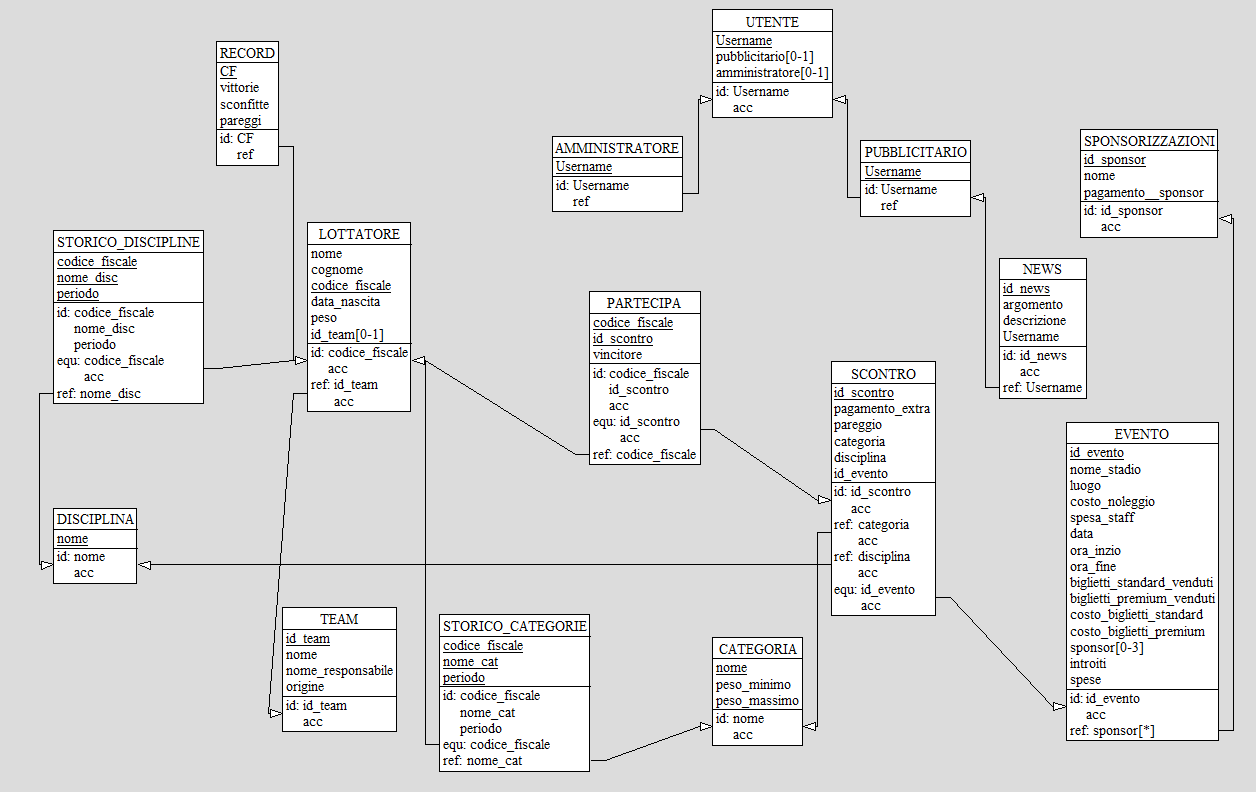
\includegraphics[scale=0.7, angle=90]{./img/schema_rel_finale.png}

\section{Traduzione operazioni in query SQL}
\subsection{Creazione tabelle}
\begin{verbatim}
CREATE TABLE AMMINISTRATORE (
    username varchar(30) NOT NULL PRIMARY KEY
);

CREATE TABLE LOTTATORE ( 
    codiceFiscale varchar(50) NOT NULL,
    nome varchar(20) NOT NULL,
    cognome varchar(30) NOT NULL,
    dataNascita date NOT NULL,
    team varchar(40), 
    peso float NOT NULL, 
    categoria varchar(20) NOT NULL,
    arteMarziale ENUM('BJJ', 'MMA', 'MuayThai') NOT NULL, 
    PRIMARY KEY (codiceFiscale) 
); 

CREATE TABLE TEAM (
    idTeam integer NOT NULL,
    nome varchar(50) NOT NULL,
    nome_responsabile varchar(20),
    origine varchar(40),
    PRIMARY KEY (idTeam)
);

CREATE TABLE RECORD (
    codiceFiscale varchar(50) NOT NULL,
    vittorie integer,
    sconfitte integer,
    pareggi integer,
    PRIMARY KEY (codiceFiscale)
);

CREATE TABLE CLASSIFICA_PIUMA (
    codiceFiscale varchar(50) NOT NULL,
    nome varchar(20) NOT NULL,
    cognome varchar(30) NOT NULL,
    peso float NOT NULL,
    arteMarziale ENUM('BJJ', 'MMA', 'MuayThai') NOT NULL,
    PRIMARY KEY (codiceFiscale)
);

CREATE TABLE CLASSIFICA_WELTERWEIGHT (
    codiceFiscale varchar(50) NOT NULL,
    nome varchar(20) NOT NULL,
    cognome varchar(30) NOT NULL,
    peso float NOT NULL,
    arteMarziale ENUM('BJJ', 'MMA', 'MuayThai') NOT NULL,
    PRIMARY KEY (codiceFiscale)
);

CREATE TABLE CLASSIFICA_MEDIO (
    codiceFiscale varchar(50) NOT NULL,
    nome varchar(20) NOT NULL,
    cognome varchar(30) NOT NULL,
    peso float NOT NULL,
    arteMarziale ENUM('BJJ', 'MMA', 'MuayThai') NOT NULL,
    PRIMARY KEY (codiceFiscale)
);

CREATE TABLE CLASSIFICA_MASSIMI (
    codiceFiscale varchar(50) NOT NULL,
    nome varchar(20) NOT NULL,
    cognome varchar(30) NOT NULL,
    peso float NOT NULL,
    arteMarziale ENUM('BJJ', 'MMA', 'MuayThai') NOT NULL,
    PRIMARY KEY (codiceFiscale)
);

CREATE TABLE DISCIPLINA (
    nome ENUM('BJJ','MMA','MuayThai') PRIMARY KEY
);

CREATE TABLE CATEGORIA (
    nome ENUM('PesoPiuma','Welterweight',
            'PesoMedio','PesiMassimi') PRIMARY KEY,
    pesoMinimo integer,
    pesiMassimi integer 
);

CREATE TABLE SCONTRO (
    idEvento integer NOT NULL,
    idScontro integer NOT NULL,
    disciplina ENUM('BJJ','MMA','MuayThai'),
    categoria ENUM('PesoPiuma','Welterweight',
                    'PesoMedio','PesiMassimi'),
    pagamentoExtra float,
    PRIMARY KEY (idEvento, idScontro)
);

CREATE TABLE STORICO_SCONTRI (
    idEvento integer NOT NULL,
    idScontro integer NOT NULL,
    primoPartecipante varchar(50) NOT NULL,
    secondoPartecipante varchar(50) NOT NULL,
    vincitore varchar(50),
    perdente varchar(50),
    pareggio bool,
    PRIMARY KEY (idScontro, idEvento),
    CONSTRAINT PAREGGIO CHECK 
        ((pareggio IS TRUE AND vincitore IS NULL 
        AND perdente IS NULL) OR
        (pareggio IS FALSE AND vincitore IS NOT NULL 
        AND perdente IS NOT NULL))
);

CREATE TABLE EVENTO (
    idEvento integer NOT NULL,
    nomeStadio varchar(40) NOT NULL,
    luogo varchar (50) NOT NULL,
    costoNoleggio float,
    spesaStaff float,
    dataEvento date NOT NULL,
    oraInizio varchar(10) NOT NULL,
    oraFine varchar(10) NOT NULL,
    bigliettiStandardVenduti integer,
    bigliettiPremiumVenduti integer,
    costoBigliettiPremium integer,
    costoBigliettiStandard integer,
    sponsor JSON,
    PRIMARY KEY (idEvento),
    CONSTRAINT ORARIO CHECK (oraInizio <= oraFine)
);

CREATE TABLE SPONSORIZZAZIONI (
    idSponsor integer NOT NULL,
    nome varchar(40) NOT NULL,
    pagamentoSponsor float,
    PRIMARY KEY (idSponsor)
);

CREATE TABLE STORICO_EVENTI (
    idEvento integer NOT NULL,
    introiti float,
    spese float,
    guadagniComplessivi float,
    PRIMARY KEY (idEvento)
);
\end{verbatim}
\subsection{Operazioni amministratore}
\subsubsection{Aggiungere lottatore}
\begin{verbatim}
INSERT INTO LOTTATORE (nome, cognome, codiceFiscale, 
    dataNascita, team, peso, categoria, arteMarziale)
VALUES (?, ?, ?, ?, ?, ?, ?, ?);

-- Aggiungere Record --

INSERT INTO RECORD (idRecord, vittorie, sconfitte, pareggi)
VALUES (?, 0, 0, 0);

-- Aggiungere classifica --

INSERT INTO CLASSIFICA (nome, cognome, codiceFiscale, peso, 
    arteMarziale)
VALUES (?, ?, ?, ?, ?);

\end{verbatim}
\textsl{P.S: In questo caso inserisco il lottatore nella tabella 'classifica' che non esiste per comodità, 
nell'applicazione invece sarà presente un controllo che farà in modo che il partecipante venga 
inserito nella classifica giusta in base al suo peso.}

\subsubsection{Rimuovere lottatore}
\begin{verbatim}
DELETE FROM LOTTATORE
WHERE codiceFiscale = ?

-- Elimina il record corrispondente --

DELETE FROM RECORD
WHERE codiceFiscale = ?

-- Elimina l'elemento in classifica

DELETE FROM CLASSIFICA
WHERE codiceFiscale = ?
\end{verbatim}
\textsl{P.S: vale la stessa cosa che ho detto prima per l'aggiunta classifica.}
\subsubsection{Aggiungere team}
\begin{verbatim}
INSERT INTO TEAM (idTeam, nome, nome_responsabile, origine)
VALUES(?, ?, ?, ?);
\end{verbatim}
\subsubsection{Rimuovere team}
\begin{verbatim}
DELETE FROM TEAM 
WHERE idTeam = ?
\end{verbatim}
\subsubsection{Aggiungere sponsor}
\begin{verbatim}
INSERT INTO SPONSORIZZAZIONI(idSponsor, nome, pagamentoSponsor)
VALUES (?, ?, ?);
\end{verbatim}
\subsubsection{Rimuovere sponsor}
\begin{verbatim}
DELETE FROM SPONSORIZZAZIONI
WHERE idSponsor = ?
\end{verbatim}
\subsubsection{Registrare evento}
\begin{verbatim}
INSERT INTO EVENTO (idEVento, nomeStadio, luogo, costoNoleggio,
    spesaStaff, dataEvento, oraInizio, oraFine, 
    bigliettiStandardVenduti, bigliettiPremiumVenduti, 
    costoBigliettiStandard, costoBigliettiPremium, sponsor)
VALUES (?, ?, ?, ?, ?, ?, ?, ?, ?, ?, ?, ?, ?);

-- Inserire evento in storicoEventi --

INSERT INTO STORICO_EVENTI (idEvento, introiti, spese, 
    guadagniComplessivi)
VALUES (?, ?, ?, ?);

-- Aggiungere Scontro (2-5 volte, in base al tipo di evento) --

INSERT INTO SCONTRO (idEvento, idScontro, disciplina, 
    categoria, pagamentoExtra)
VALUES (?, ?, ?, ?, ?);

-- Inserire Scontro nello storicoScontri --

INSERT INTO STORICO_SCONTRI (idEvento, idScontro, 
    primoPartecipante, secondoPartecipante, vincitore, 
    perdente, pareggio)
VALUES (?, ?, ?, ?, ?, ?, ?);
\end{verbatim}
\subsubsection{Modificare lottatore}
\begin{verbatim}

UPDATE LOTTATORE 
SET nome = ?, cognome = ?,
    dataNascita = ?, team = ?, 
    peso = ?, categoria = ?, 
    arteMarziale = ?
WHERE codiceFiscale = ?

UPDATE RECORD 
SET vittore = ?,
    sconfitte = ?,
    pareggi = ?
WHERE codiceFiscale = ?
    
\end{verbatim}
\subsubsection{Visualizzare classifiche}
\begin{verbatim}
SELECT c.codicFiscale
FROM CLASSIFICA c
JOIN RECORD r ON c.codiceFiscale = r.codiceFiscale
ORDER BY (r.vittoria * 3 + r.pareggio) DESC;
    
\end{verbatim}

\chapter{Progettazione dell'applicazione}
\section{Descrizione dell'architettura dell'applicazione realizzata}
L'applicazione che permette di gestire il database è stata creata utilizzando \textrm{Typescript} in combinazione con il framework 
\emph{React}, mentre per quanto riguarda il database, esso risiede in locale ed è stato sviluppato usando \emph{MySQL}.
L'applicazione è un'applicazione web che si appoggia a un server locale. Essa consente quindi la possibilità di connettere 
frontend e backend utilizzando il protocollo \textbf{HTTP}, e quindi attraverso delle \textbf{API REST}. Grazie a un server locale, 
il backend avrà la possibilità di ricevere richieste dal frontend, portando con sé parametri e restituendo valori, il tutto 
evitando una connessione diretta tramite codice. Questo design permette all'applicazione di avere una scalabilità maggiore, eliminando 
eventuali dipendenze tra frontend e backend. Inoltre, per la gestione del database da parte del backend, si utilizza la libreria 
\emph{TypeORM} di \textrm{Typescript}. Libreria che permette di eseguire operazioni sui dati mediante codice.

\begin{figure}
    \centering
    \includegraphics[scale=0.3]{./img/menù_iniziale.png}
    \caption{\textit{Menù iniziale dell'applicazione}}
    \medskip
    In questo menù sarà possibile accedere alle operazioni di gestione del database(es: \ref{addEvento} per la registrazione di un evento) 
    oppure alle classifiche generali dei lottatori \ref{categoria}.
\end{figure}

\begin{figure}
    \centering
    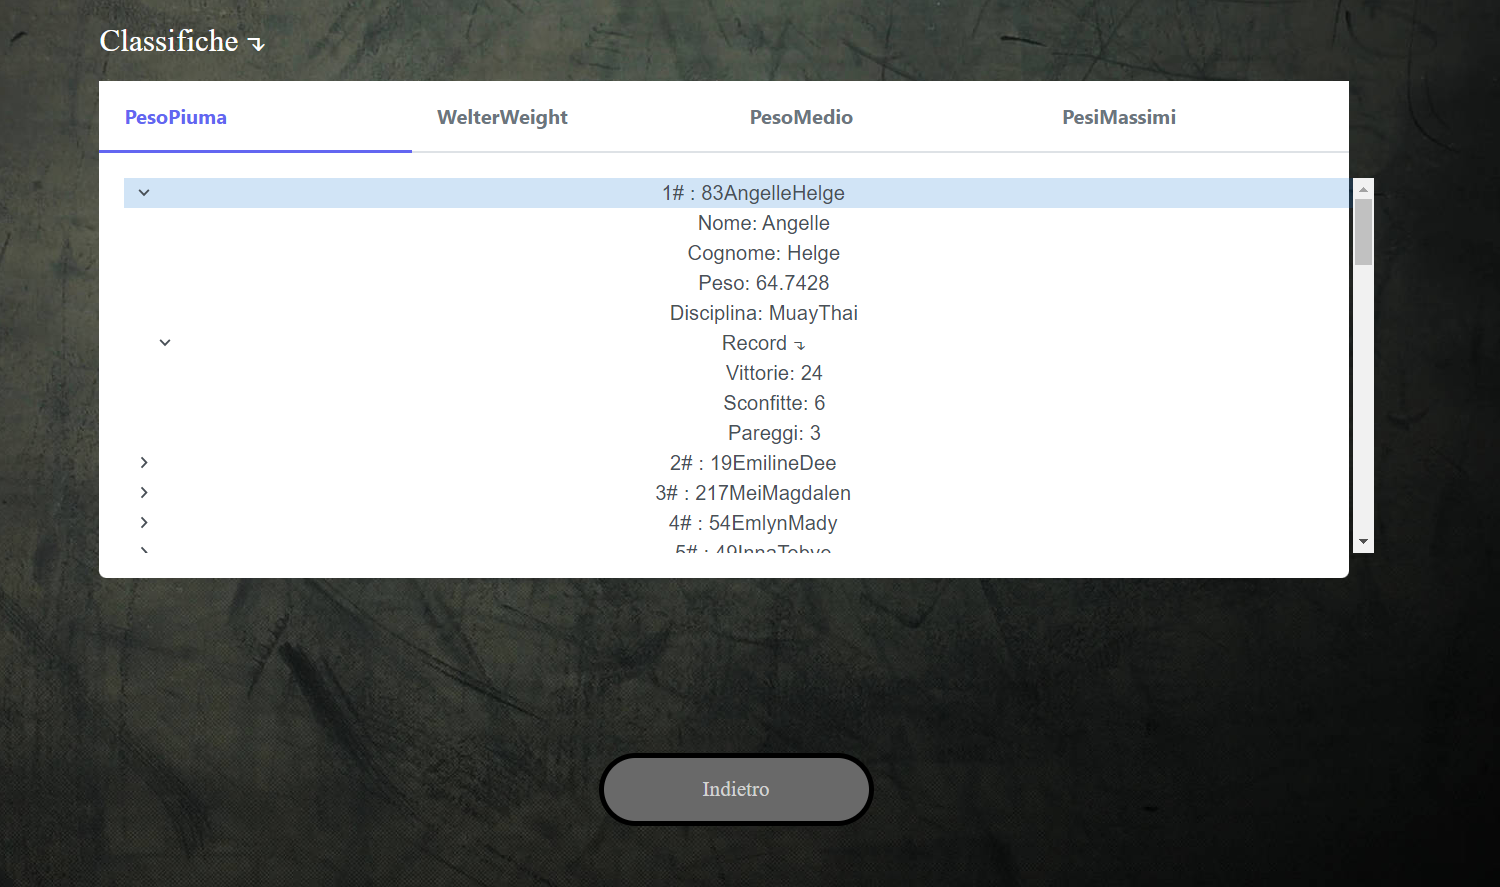
\includegraphics[scale=0.4]{./img/classifiche.png}
    \caption{\textit{Classifiche di tutti i partecipanti divisi in categorie}}
    \label{categoria}
\end{figure}

\begin{figure}
    \centering
    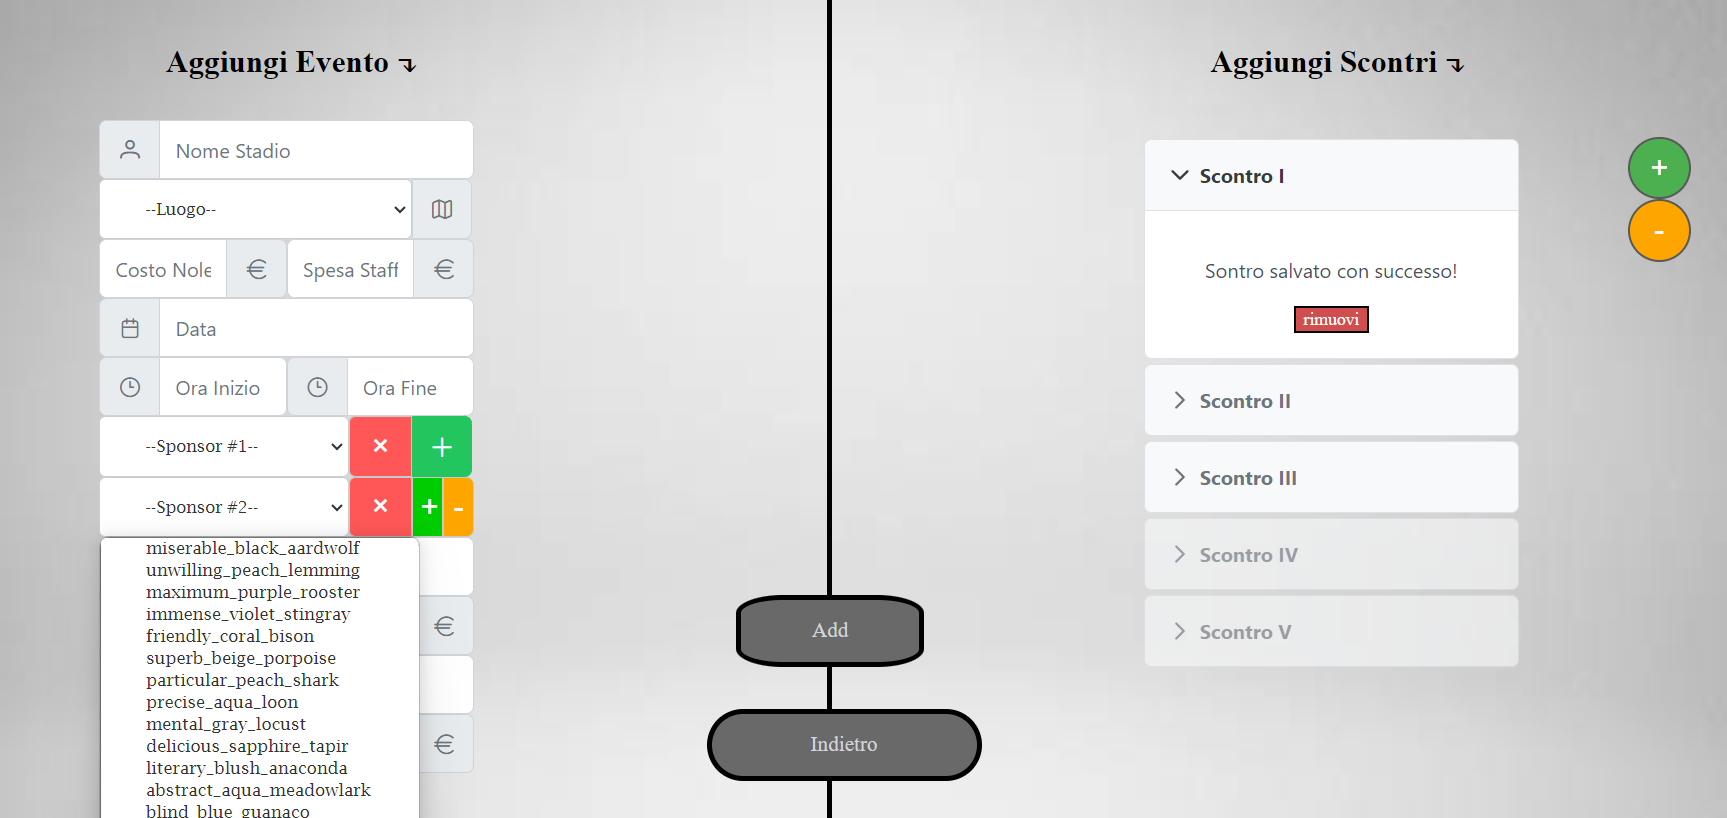
\includegraphics[scale=0.35]{./img/eventoAdd.png}
    \caption{\textit{Pagina che permette di registrare un evento e i proprio scontri}}
    \medskip
    Come si puo notare dall'immagine qua abbiamo una schermata dove è possibile registrare Eventi inserendo tutti i dati necessari nella 
    parte sinistra dello schermo, nella parte destra invece potremmo aggiungere da 2 a 5 scontri (in questo caso notiamo che 
    uno è già stato aggiunto e ci viene proposta la possibilità di rimuoverlo e modificarlo se desiderato).
    \label{addEvento}
\end{figure}

\begin{figure}
    \centering
    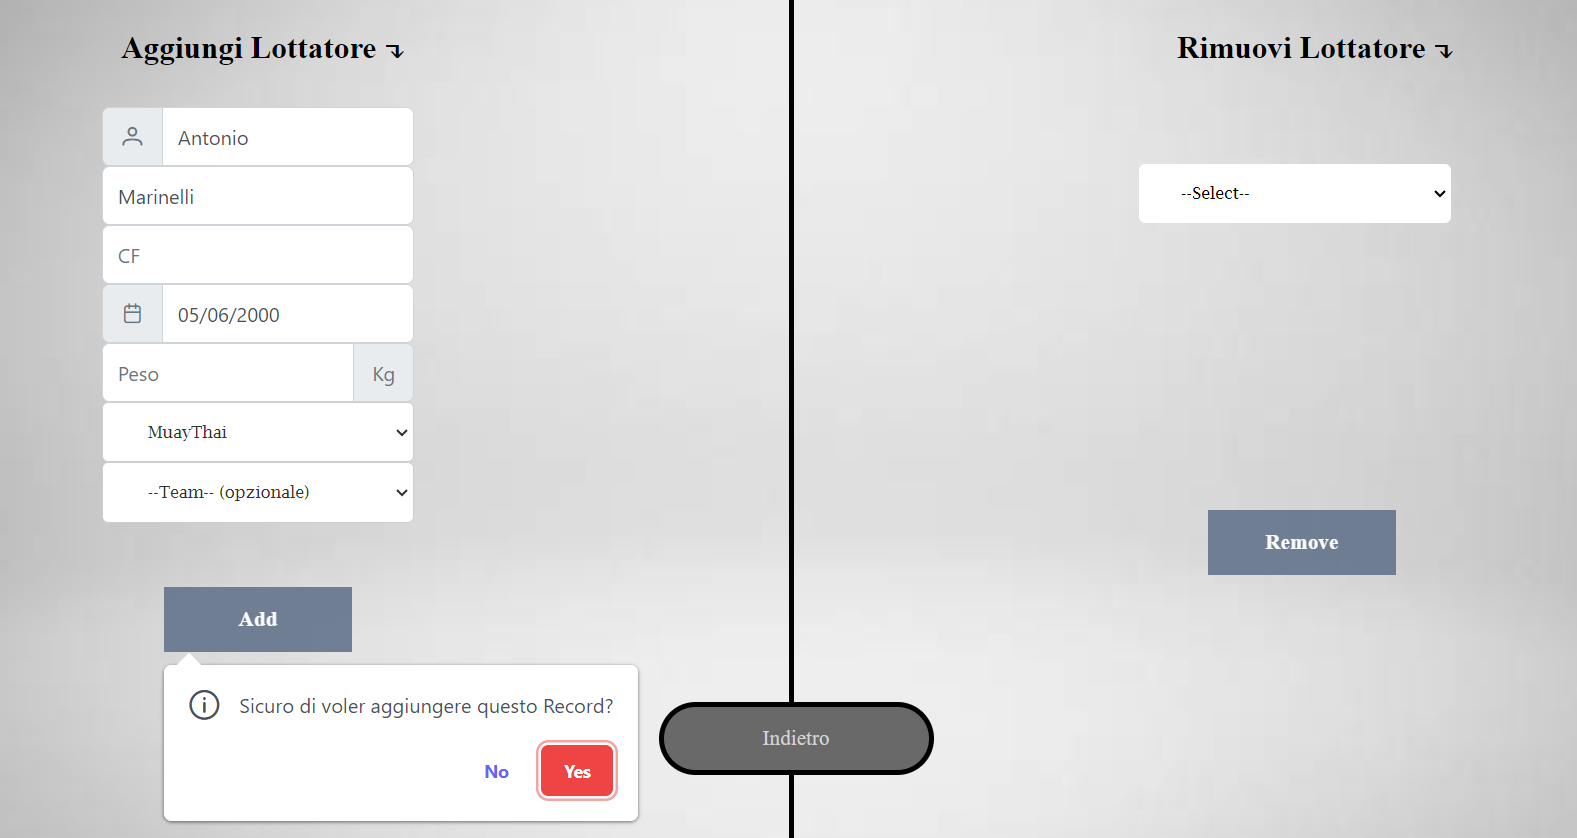
\includegraphics[scale=0.4]{./img/AddLottatore.png}
    \caption{\textit{Pagina che ci permette di aggiungere e rimuovere lottatori}}
\end{figure}



\end{document}
